\documentclass{standalone}
\usetikzlibrary{positioning, shapes.geometric, arrows.meta, calc}
%\begin{document}
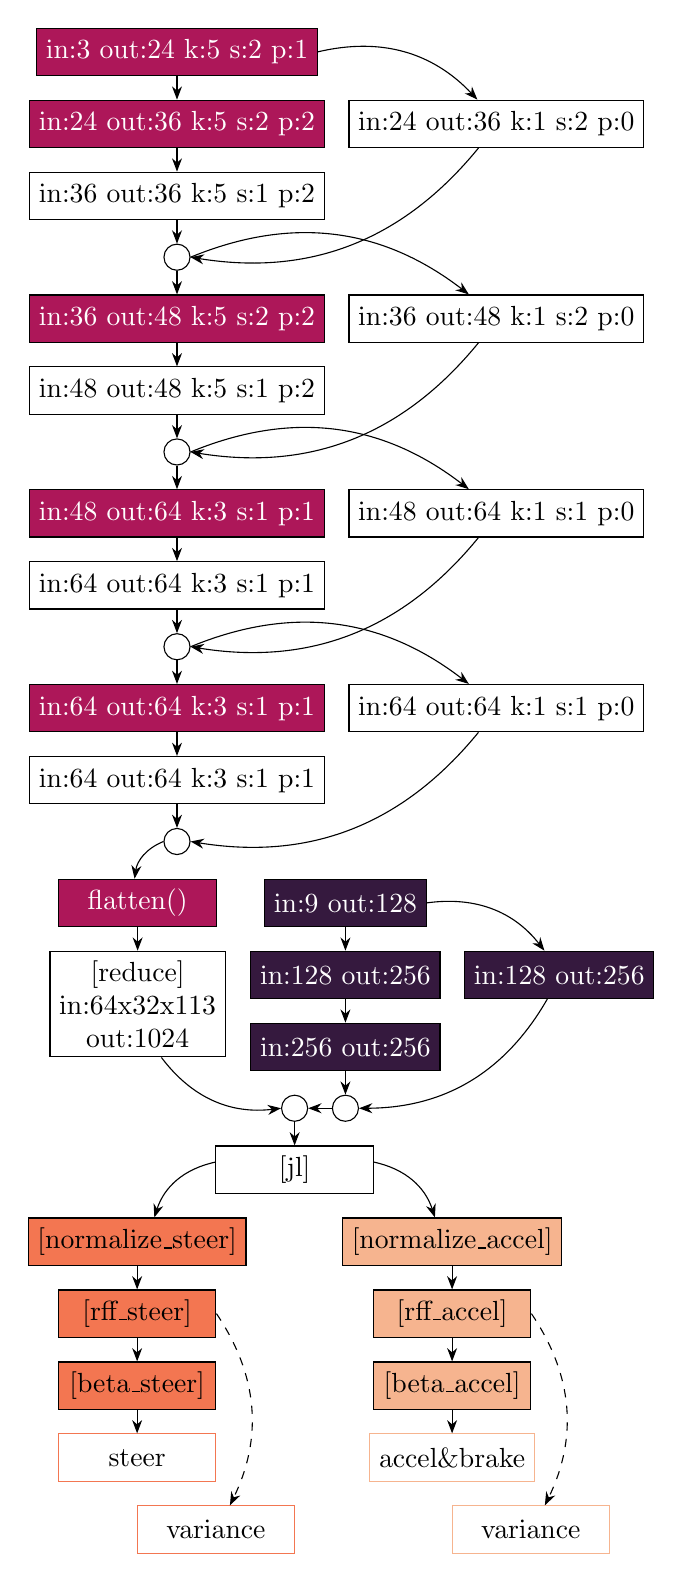
\begin{tikzpicture}[
    node distance=0.3cm and 0.3cm,
    every node/.style={draw, rectangle, minimum height=0.6cm, minimum width=2cm, align=center},
    %davenode/.style={rectangle, draw=red!60},
    arrow/.style={-Stealth}
]

% Colors
\definecolor{plum}{RGB}{53, 25, 62} % measurement encoder
\definecolor{pink}{RGB}{173, 23, 89} % layers taken from dave2
\definecolor{orange}{RGB}{243, 118, 81} % GP steer
\definecolor{sand}{RGB}{246, 180, 143} % GP accel

% Nodes
\node (first) [fill=pink] {\textcolor{white}{in:3 out:24 k:5 s:2 p:1}};

\node (second_i) [below=of first, fill=pink] {\textcolor{white}{in:24 out:36 k:5 s:2 p:2}};
\node (second_h) [below=of first, right=of second_i] {in:24 out:36 k:1 s:2 p:0};
\node (second_o) [below=of second_i] {in:36 out:36 k:5 s:1 p:2};

\node (c2) [draw, circle, minimum size=0.3cm, below=of second_o]{};

\node (third_i) [below=of c2, fill=pink] {\textcolor{white}{in:36 out:48 k:5 s:2 p:2}};
\node (third_h) [below=of c2, right=of third_i] {in:36 out:48 k:1 s:2 p:0};
\node (third_o) [below=of third_i] {in:48 out:48 k:5 s:1 p:2};

\node (c3) [draw, circle, minimum size=0.3cm, below=of third_o] {};

\node (fourth_i) [below=of c3, fill=pink] {\textcolor{white}{in:48 out:64 k:3 s:1 p:1}};
\node (fourth_h) [below=of c3, right=of fourth_i] {in:48 out:64 k:1 s:1 p:0};
\node (fourth_o) [below=of fourth_i] {in:64 out:64 k:3 s:1 p:1};

\node (c4) [draw, circle, minimum size=0.3cm, below=of fourth_o] {};

\node (fifth_i) [below=of c4, fill=pink] {\textcolor{white}{in:64 out:64 k:3 s:1 p:1}};
\node (fifth_h) [below=of c4, right=of fifth_i] {in:64 out:64 k:1 s:1 p:0};
\node (fifth_o) [below=of fifth_i] {in:64 out:64 k:3 s:1 p:1};

\node (c5) [draw, circle, minimum size=0.3cm, below=of fifth_o] {};

\node (flatten) [below=of c5, xshift=-0.5cm, fill=pink] {\textcolor{white}{flatten()}};
\node (reduce) [below=of flatten] {[reduce]\\in:64x32x113\\out:1024};

\node (first_m) [right=of flatten, fill=plum, xshift=0.3cm] {\textcolor{white}{in:9 out:128}};
\node (m_i) [below=of first_m, fill=plum] {\textcolor{white}{in:128 out:256}};
\node (m_h) [below=of first_m, right=of m_i, fill=plum] {\textcolor{white}{in:128 out:256}};
\node (m_o) [below=of m_i, fill=plum] {\textcolor{white}{in:256 out:256}};

\node (cm) [draw, circle, minimum size=0.3cm, below=of m_o] {};
\node (c) [draw, circle, minimum size=0.3cm, left=of cm] {};

\node (jl) [below=of c] {[jl]};

\node (norm_s) [below=of jl, xshift=-2cm, fill=orange] {[normalize\_steer]};
\node (rff_s) [below=of norm_s, fill=orange] {[rff\_steer]};
\node (beta_s) [below=of rff_s, fill=orange] {[beta\_steer]};
\node (pred_s) [draw=orange, below=of beta_s] {steer};
\node (var_s) [draw=orange, below=of pred_s, xshift=1cm] {variance};

\node (norm_a) [below=of jl, xshift=2cm, fill=sand] {[normalize\_accel]};
\node (rff_a) [below=of norm_a, fill=sand] {[rff\_accel]};
\node (beta_a) [below=of rff_a, fill=sand] {[beta\_accel]};
\node (pred_a) [draw=sand, below=of beta_a] {accel\&brake};
\node (var_a) [draw=sand, below=of pred_a, xshift=1cm] {variance};

% Edges
\draw[arrow] (first) to (second_i);
\draw[arrow, bend left] (first.east) to (second_h);
\draw[arrow] (second_i) to (second_o);
\draw[arrow, bend left] (second_h) to (c2.east);
\draw[arrow] (second_o) to (c2);
\draw[arrow] (c2) to (third_i);

\draw[arrow, bend left] (c2.east) to (third_h);
\draw[arrow] (third_i) to (third_o);
\draw[arrow, bend left] (third_h) to (c3.east);
\draw[arrow] (third_o) to (c3);
\draw[arrow] (c3) to (fourth_i);

\draw[arrow, bend left] (c3.east) to (fourth_h);
\draw[arrow] (fourth_i) to (fourth_o);
\draw[arrow, bend left] (fourth_h) to (c4.east);
\draw[arrow] (fourth_o) to (c4);
\draw[arrow] (c4) to (fifth_i);

\draw[arrow, bend left] (c4.east) to (fifth_h);
\draw[arrow] (fifth_i) to (fifth_o);
\draw[arrow, bend left] (fifth_h) to (c5.east);
\draw[arrow] (fifth_o) to (c5);

\draw[arrow, bend right] (c5.west) to (flatten);
\draw[arrow] (flatten) to (reduce);
\draw[arrow] (first_m) to (m_i);
\draw[arrow, bend left] (first_m.east) to (m_h);
\draw[arrow] (m_i) to (m_o);
\draw[arrow] (m_o) to (cm);
\draw[arrow, bend left] (m_h) to (cm.east);

\draw[arrow, bend right] (reduce) to (c.west);
\draw[arrow] (cm.west) to (c.east);
\draw[arrow] (c) to (jl);

\draw[arrow, bend right] (jl) to (norm_s);
\draw[arrow] (norm_s) to (rff_s);
\draw[arrow] (rff_s) to (beta_s);
\draw[arrow, dashed, bend left] (rff_s.east) to (var_s);
\draw[arrow] (beta_s) to (pred_s);

\draw[arrow, bend left] (jl) to (norm_a);
\draw[arrow] (norm_a) to (rff_a);
\draw[arrow] (rff_a) to (beta_a);
\draw[arrow, dashed, bend left] (rff_a.east) to (var_a);
\draw[arrow] (beta_a) to (pred_a);

\end{tikzpicture}
%\end{document}